\capitulo{3}{Conceptos teóricos}

La parte del proyecto con evidente carga teórica es la fase de investigación. En el apéndice del cuaderno de investigación se explica el uso de todas las técnicas que hemos empleado en los experimentos, especificando implementaciones concretas, parámetros utilizados y resultados obtenidos. En este apartado se van a exponer los conceptos teóricos en los que se basan esas técnicas sin entrar en los detalles de implementación.  

Dado que el desarrollo de la investigación se ha basado en el proceso \textit{KDD} (explicado más detenidamente en el apartado de Técnicas y Herramientas), este apartado se estructurará en función de los pasos que incluye este proceso: 

\section{Limpieza de datos}

Los datos de los que disponemos tienen los siguientes atributos: 

\begin{itemize}
	\item \textbf{MAC\_NGMATT} y \textbf{UUID\_BSN}: identificador del colchón asociado alos tubos de presión e identificador del sensor de biométricas respectivamente. 
	\item \textbf{DateTime}: día y hora en la que fue tomada cada instancia de dato. 
	\item \textbf{P1, P2, P3, P4, P5, P6, P7, P8, P9, P10, P11, P12}: presiones, en mBar, captadas por los 12 tubos de presión integrados en el colchón. 
	\item \textbf{HR, RR, SV, HRV, B2B}: valores de las constantes vitales que corresponden con la frecuencia cardíaca (pulsaciones/minuto), la frecuencia respiratoria (respiraciones/minuto), el volumen sistólico (mililitros), la variabilidad del ritmo cardíaco (milisegundos) y el tiempo entre pulsaciones (milisegundos) respectivamente. 
	\item \textbf{SS}: potencia de la señal relativa a la matriz de tubos de presión. Un valor superior a 400 se considera aceptable. 
	\item \textbf{STATUS}: estado de medición del sensor de constantes vitales. 0=\textit{low signal}, 1=\textit{ok signal}, 2=\textit{high signal}, 3= \textit{close to overload}, 4= \textit{close to max HR}. 
\end{itemize}

Por otra parte se nos proporcionaron unos rangos aproximados de horas en los que el paciente tuvo un ataque epiléptico. 

\subsection{Eliminación de instancias por baja señal}

Dos de estos atributos, SS y STATUS, hacen referencia a la calidad de la instancia de los datos, uno haciendo referencia a la matriz de tubos de presión y otro al sensor de constantes vitales, y dado que la fase de limpieza de datos consiste en eliminar el ruido y las instancias incorrectas, es aquí donde eliminaremos todas las instancias cuyos datos no consideremos fiables en función de los valores de estos dos atributos. 

Concretamente eliminamos todas aquellas instancias que tengan un SS menor de 400, pero no tendremos en cuenta el valor de STATUS ya que, como se explicará más adelante, los valores de las constantes vitales no se han usado para la búsqueda del modelo de clasificación.

\subsection{Eliminación manual del ruido}

Mediante una inspección inicial de los datos se detectó que algunos datos de los tubos de presión en ocasiones eran negativos (lo cual no debería ocurrir), y aparecían valores bajos de presión en momentos en los que la cama debería estar vacía. Por esta razón, se decidió considerar todo valor de presión menor a 5 como ruido convirtiéndolo a 0 (de esta forma nos deshacemos también de los valores negativos). 

\subsection{Filtrado}

Otra forma de eliminar el ruido de una señal consiste en usar filtros. Un filtro es un sistema que se aplica a una señal (en nuestro caso la señal de presiones en el tiempo) y la transforma para conseguir un objetivo concreto, en este caso el suavizado de la señal para eliminar el ruido. Se han probado dos tipos de filtro distintos: 

\begin{itemize}
	\item \textbf{Filtro de Butterworth}: Diseñado para filtrado de señales eléctricas, trata de producir la respuesta más plana que sea posible hasta la frecuencia de corte (\textit{Wn}), dicho de otra forma, trata de mantener intactas las frecuencias por debajo de la frecuencia de corte mientras disminuye las frecuencias superiores con razón proporcional a \textit{N}, siendo \textit{N} el orden de filtrado:
	\begin{center}
		$|H| = \dfrac{1}{\sqrt{1+(W/Wn)^{2N}}}$
	\end{center}

	\begin{figure}[H]
		\centering
		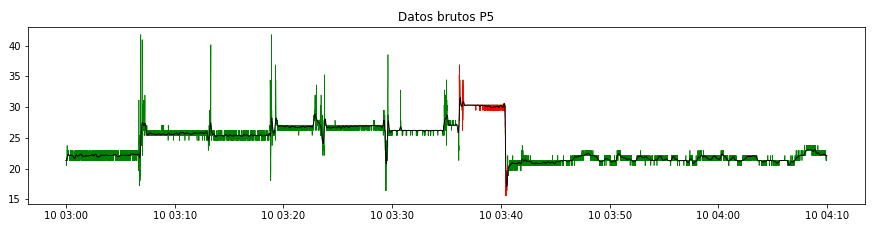
\includegraphics[width=1\textwidth]{../img/senalP5butter.png}
		\caption{Ejemplo de señal de presión (P5) filtrada mediante un filtro de Butterworth con \textit{N}=3 y \textit{Wn}=0.05. En verde la señal original y en negro la señal filtrada.}
		\label{fig:senalP5butter}
	\end{figure}
	
	\item \textbf{Filtro de Savitzky–Golay}: Se basa en el cálculo de una regresión polinomial local para la que se debe especificar un tamaño de ventana (\textit{window\_lenght}) y el orden del polinomio utilizado en la regresión (\textit{polyorder}). 
	
	\begin{figure}[H]
		\centering
		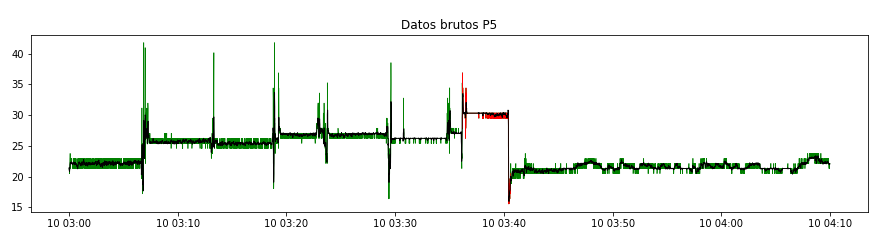
\includegraphics[width=1\textwidth]{../img/senalP5savgol.png}
		\caption{Ejemplo de señal de presión (P5) filtrada mediante un filtro de Svatzky-Golay con \textit{window\_length}=15 y \textit{polyorder}=2. En verde la señal original y en negro la señal filtrada}
		\label{fig:senalP5savgol}
	\end{figure}
\end{itemize}

\subsection{Eliminación de atributos inconsistentes}

En la primera inspección de los datos también se advirtió que los atributos referentes a las constantes vitales eran nulos de forma intermitente y en una gran cantidad de las instancias. Esto se debió al mal funcionamiento del sensor durante las primeras etapas de recogida de los datos. 

Aunque muchas técnicas de minería de datos soportan la presencia de atributos desconocidos (\textit{missing}) en algunas de las instancias, la cantidad de instancias con constantes vitales nulas o incorrectas era tan grande que se tomó la decisión de no tener en cuenta estos datos para el resto de experimentos.  

Cabe destacar que esto supone un gran inconveniente, ya que la mayoría de técnicas de detección automática encontrados en el estado del arte (quitando las centradas en EEG) se basan en datos biométricos. 

\section{Integración de datos}

Los datos disponibles corresponden con las instancias recogidas al lo largo de varios meses de una sola cama (un solo paciente). Estos datos nos han sido proporcionados en varios archivos de extensión .csv, por lo que la fase de integración ha consistido en recoger los datos en varios subconjuntos (varios DataFrames de Pandas), uno por cada noche, considerando que una noche corresponde con el periodo de tiempo en el que el paciente estuvo acostado en la cama de forma ininterrumpida. 

\section{Selección de datos}

La selección de los datos consiste en desechar aquellos atributos o instancias que no resultan útiles para la extracción de conocimiento. A estas alturas del proceso seguimos teniendo datos relativos a la identificación del colchón, a la hora en la que se tomó la instancia de dato y a las presiones. 

\subsection{Eliminación de identificadores}

Al contar con los datos de un único paciente, los atributos de identificación de la cama MAC\_NGMATT y UUID\_BSN no proporcionan ningún tipo de información útil para la extracción de conocimiento, por lo que ni siquiera son tenidos en cuenta en la fase de integración. 

\subsection{Eliminación de atributos de baja variabilidad}

Este proceso consiste en detectar aquellos atributos que varían menos de un umbral determinado durante el tiempo, y por lo tanto no proporcionarán información relevante. 

Tras llevar a cabo este proceso se eliminaron los atributos P7, P8, P9, P10, P11 y P12. Esto tiene sentido ya que esos campos corresponden con la matriz de tubos de presión de una de las mitades del modelo de colchón de matrimonio, y el colchón con el que se trabaja en este proyecto es individual. 

En este punto ya hemos seleccionado los atributos que serán considerados como \textbf{Datos en Bruto}: 
\begin{itemize}
	\item DateTime
	\item P1, P2, P3, P4, P5 y P6
\end{itemize}

\section{Transformación de datos}

TODO

\section{Minería de datos}

TODO

\section{Evaluación de patrones}

TODO

\section{Presentación del conocimiento}

TODO
